\documentclass{article}

% Language setting
% Replace `english' with e.g. `spanish' to change the document language
\usepackage[spanish]{babel}

% Set page size and margins
% Replace `letterpaper' with `a4paper' for UK/EU standard size
\usepackage[letterpaper,top=2cm,bottom=2cm,left=3cm,right=3cm,marginparwidth=1.75cm]{geometry}

% Useful packages
\usepackage{amsmath}
\usepackage{graphicx}
\usepackage{enumitem}
\usepackage{comment}
\usepackage{wrapfig}
\usepackage[colorlinks=true, allcolors=blue]{hyperref}
\usepackage{subcaption}

\title{AED Tema 4. Árboles de busca equilibrados (AVL)}
\author{Martín González Dios
\href{https://github.com/martindios}{\includegraphics[height=0.5cm]{github.png}}}
\date{}

\begin{document}
\maketitle

Con árboles desbalanceados se pierde la eficiencia de búsqueda, acercándose a la de una lista, es
decir O(n) para la búsqueda. Sin embargo, con árboles equilibrados se consigue una eficiencia
de O(log(n)) en la búsqueda, inserción o eliminación. \\

Aquellos árboles que se mantienen siempre equilibrados debido a constantes reordenaciones
se conocen como \textbf{árboles AVL} (Adelson-Velskii y Landis). \\

En este tipo de árboles, cada nodo cuenta con un campo llamado \textbf{factor de equilibrio},
que almacena la diferencia entre la altura del subárbol derecho y la altura del subárbol izquierdo
para dicho nodo. Como se estudió en el tema 2, el árbol será equilibrado mientras el valor
absoluto de todos los factores de carga sea \textbf{menor que 2}.

\section{Inserción}
Se pueden dar varios casos en la inserción:
\begin{itemize}
    \item Si las ramas izquiereda y derecha tienen la misma altura, da igual donde se inserte, que al insertar solo se producirá un nuevo factor de equilibrio de -1 o 1, con lo que el árbol sigue estando equilibrado.

    \item Si las ramas izquierda y derecha difieren en su altura en 1 unidad:
        \begin{itemize}
            \item Si el factor de equilibrio era -1 y se inserta por la derecha, o si el factor de equilibrio era 1 y se inserta por la izquierda, el nuevo factor de equilibrio pasa a ser 0, por lo que se mejora el equilibrio del árbol y no hay ningún problema.

            \item Si el factor de equilibrio era -1 y se inserta por la izquierda, o si el factor de equilibrio era 1 y se inserta por la derecha, el nuevo factor de equilibrio pasa a ser -2 o 2 (respectivamente), \textbf{desequilibrando el árbol}, y siendo necesaria una \textbf{reestructuración}.
        \end{itemize}
\end{itemize}

\newpage

\section{Reestructuración}
Tras una inserción, el nodo insertado pasa a ser un nodo hoja, por lo que su factor de equilibrio
es 0. Posteriormente vamos subiendo por el árbol recalculando los factores de equilibrio hasta
encontrar uno cuyo valor absoluto sea 2, a partir del cual habrá que reestructurar el árbol. Este proceso se repite hasta llegar al nodo raíz. \\

Existen 4 tipos de estructuraciones, que no son más que rotaciones del árbol: I significa izquierda y D derecha.

\begin{itemize}
    \item \textbf{Rotación simple II}: se produce cuando un nodo tiene factor -2 y su hijo izquierdo, factor -1. Se rota hacia la derecha, dejando el nodo con factor -1 como nuevo padre, el nodo con factor -2 como hijo derecho, y el nodo que originó el desequilibrio, como hijo izquierdo.

    \item \textbf{Rotación simple DD}: se produce cuando un nodo tiene factor 2 y su hijo derecho, factor -1. Es lo contrario al caso anterior: rotación a la izquierda, nodo con factor 1 como padre, nodo con factor 2 como hijo izquierdo, y nodo que origin´o el desequilibrio como hijo derecho.

    \item \textbf{Rotación compuesta DI}: se produce cuando un nodo tiene factor 2 y su hijo derecho, factor -1. Se rota el hijo con factor a la derecha y se sube el nodo que originó el desequilibrio a su posición, y se tiene una rotación simple DD.

    \item \textbf{Rotación comuesta ID}: se produce cuando un nodo tiene factor -2 y su hijo izquierdo, factor 1. Se rota el hijo con factor 1 a la izquierda y se pone el nodo que causó el desequilibrio en su posición, teniendo un rotación simple II.
\end{itemize}

\begin{figure}[h]
    \centering
    \begin{subfigure}{0.45\textwidth}
        \centering
        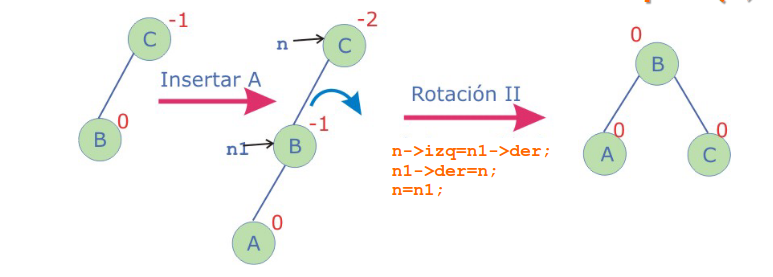
\includegraphics[width=\linewidth]{img-t4/img_418_05.png}
        \caption{Rotación simple II}
        \label{fig:imagen1}
    \end{subfigure}
    \hfill
    \begin{subfigure}{0.45\textwidth}
        \centering
        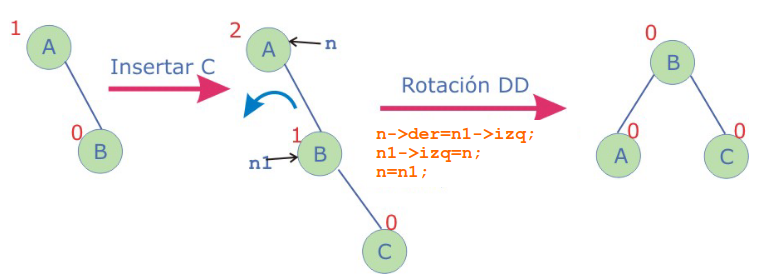
\includegraphics[width=\linewidth]{img-t4/img_079_14.png}
        \caption{Rotación simple DD}
        \label{fig:imagen2}
    \end{subfigure}
    \label{fig:imagenes}
\end{figure}

\begin{figure}[h]
    \centering
    \begin{subfigure}{0.65\textwidth}
        \centering
        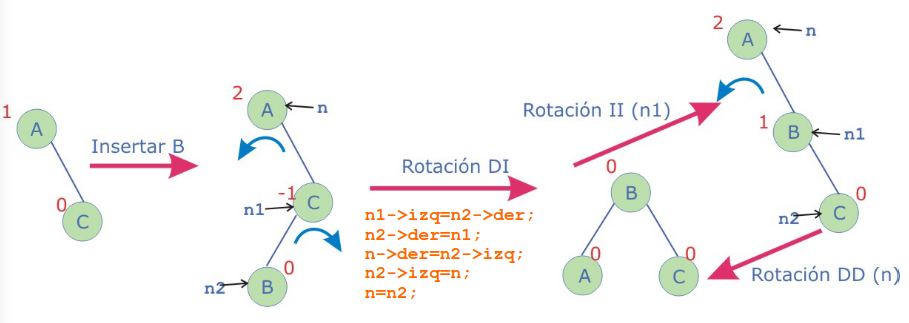
\includegraphics[width=\linewidth]{img-t4/img_591_40.png}
        \caption{Rotación compuesta DI}
        \label{fig:imagen1}
    \end{subfigure}
    \hfill
    \begin{subfigure}{0.65\textwidth}
        \centering
        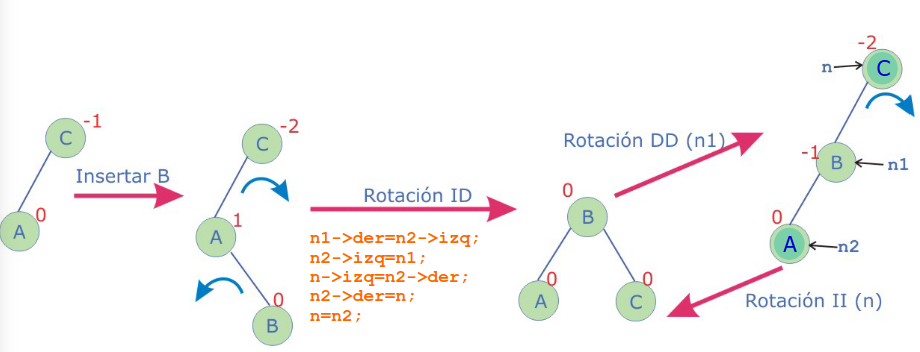
\includegraphics[width=\linewidth]{img-t4/img_376_78.png}
        \caption{Rotación compuesta ID}
        \label{fig:imagen2}
    \end{subfigure}
    \label{fig:imagenes}
\end{figure}

\newpage

\section{Eliminación}
Se sigue el \textbf{mismo algoritmo que para ABB}, pero \textbf{incluyendo las reestructuraciones necesarias}. \\
Posibles casos:
\begin{itemize}
    \item Si el nodo a suprimir es un nodo hoja, se suprime sin más.
    \item Si el nodo a suprimir solo tiene un descendiente, se sustituye por su descendiente y se elimina.
    \item Si el nodo tiene dos subárboles, se busca el nodo más a la derecha del subárbol izquierdo, o el nodo más a la izquierda del subárbol derecho, se sustituye, se elimina, y se comprueba si es necesaria reestructuración.
\end{itemize}

\end{document}
